%%%%%%%%%%%%%%%%%%%%%%%%%%%%%%%%%%%%%%%%%%%%%%%%%%%%%%%%%%%%%%%%%%%%%
% LaTeX Template: Project Titlepage Modified (v 0.1) by rcx
%
% Original Source: http://www.howtotex.com
% Date: February 2014
% 
% This is a title page template which be used for articles & reports.
% 
% This is the modified version of the original Latex template from
% aforementioned website.
% 
%%%%%%%%%%%%%%%%%%%%%%%%%%%%%%%%%%%%%%%%%%%%%%%%%%%%%%%%%%%%%%%%%%%%%%

\documentclass[12pt]{article}
\usepackage[a4paper]{geometry}
\usepackage[myheadings]{fullpage}
\usepackage{fancyhdr}
\usepackage{lastpage}
\usepackage{graphicx, wrapfig, subcaption, setspace, booktabs}
\usepackage[utf8]{inputenc}
\usepackage[T1]{fontenc}
\usepackage[font=small, labelfont=bf]{caption}
\usepackage{fourier}
\usepackage[protrusion=true, expansion=true]{microtype}
\usepackage[french]{babel}
\usepackage{caption}
\usepackage{sectsty}
\usepackage{url, lipsum}
\usepackage{amsmath}
\usepackage{amssymb}



\usepackage{tikz}
\usepackage[most]{tcolorbox}
\usepackage[pstricks]{bclogo}
\usepackage{pst-blur}




\newcommand{\HRule}[1]{\rule{\linewidth}{#1}}
\onehalfspacing
\setcounter{tocdepth}{5}
\setcounter{secnumdepth}{5}

%-------------------------------------------------------------------------------
% HEADER & FOOTER
%-------------------------------------------------------------------------------
\pagestyle{fancy}
\fancyhf{}
\setlength\headheight{15pt}
\fancyhead[L]{BTS CPRP 1}
\fancyhead[R]{Lycée Le Corbusier}
\fancyfoot[R]{Page \thepage\ sur \pageref{LastPage}}
\fancyfoot[L]{TP - Industrialisation}
%-------------------------------------------------------------------------------
% TITLE PAGE
%-------------------------------------------------------------------------------
 
 

%%%%POUR FAIRE DES EXERCICES INDÉPENDAMMENT DES SECTIONS%%%%
%%%%%%%%%%%%%%%%%%%%%%%%%%%%%%%%%%%%%%%%%%%%%%%%%%%%%%%%%%%%%%%%%%%
\newcounter{exo}
\newenvironment{exo}{\stepcounter{exo}\vspace{0.5cm}{\bfseries Question \theexo\ :}}{\par\vspace{0.5cm}}
%%%%%%%%%%%%%%%%%%%%%%%%%%%%%%%%%%%%%%%%%%%%%%%%%%%%%%%%%%%%%%%%%%%%




\begin{document}
 
\title{ 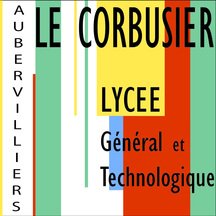
\includegraphics[width=0.18\linewidth]{Images/corbu.jpg} \hspace{2cm} \normalsize \textsc{TP Industrialisation noté \hspace{2cm} 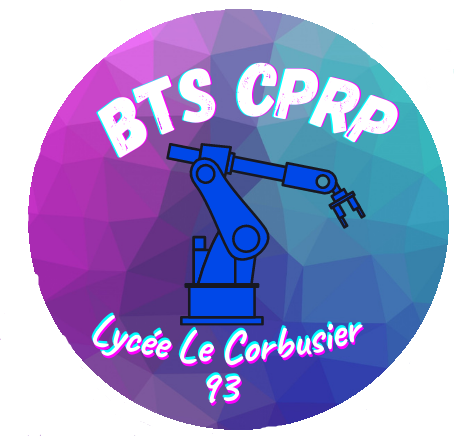
\includegraphics[width=0.2\linewidth]{Images/logo.png}}
		\\ [2.0cm]
		\HRule{0.5pt} DOSSIER SUJET \\
		\LARGE \textbf{\uppercase{TP2.1 Désignation des outils de production}}
		\HRule{2pt} \\ [0.5cm]}
\maketitle

\textbf{Deux personnes par groupe}\\
\begin{center}
Toutes les questions seront traitées dans le documents réponse fourni
\end{center}










%-------------------------------------------------------------------------------
% Section title formatting
\sectionfont{\scshape}




\newpage



%%%%%%%%%%%%%%%%%%%%%%%%%%%%%%%%%%%%%%%%%%%%%%%%%%%%%%%%%%%%%%%%
%%%%%%%%%%%%%%%% MACHINE 1 %%%%%%%%%%%%%%%%%%%%%%%%%%%%%%%%%%%%%
%%%%%%%%%%%%%%%%%%%%%%%%%%%%%%%%%%%%%%%%%%%%%%%%%%%%%%%%%%%%%%%%

\tableofcontents
\newpage



\section{Conseils pour le TP}
  \bcinfo Comme pour tous les TPs, il est conseillé de lire toutes les pages une première fois, comme pour un sujet de BTS. Vous noterez que beaucoup d'informations sont dans les annexes (comme au BTS). Certaines définitions et figures sont "en plus". Avant de poser une question, lisez bien tout le dossier. Ne perdez pas de temps, car les TPs sont conçus pour la durée entière : 3h. En plus de comprendre et apprendre, vous devrez écrire vos réponses au propre. Il vous est fortement conseillé de vous partager le travail entre vous deux. Vous ne devez cependant pas communiquer avec d'autres groupes.

\subsection{Matériel}

Crayon, crayons de couleur, stylos, règle et vos cours sont autorisés.

\subsection{Notation}
\noindent
Propreté et clarté dans les réponses : $\pm$3 points\\
Ne répondre que sur le document réponse.\\


\section{Objectifs :}
\begin{center}
\textbf{Découvrir les différents outils nécessaires à la production.}\\
\end{center}

\begin{minipage}[t]{.55\linewidth}
\textit{Compétences transversales travaillées :}
\begin{itemize}
    \item C11 : Définir et mettre en œuvre des essais réels et simulés
\end{itemize}

\end{minipage}
\begin{minipage}[t]{.44\linewidth}
\textit{Savoirs du programme travaillées :}
\begin{itemize}
    \item S5.3 – Conception des outils et porte-outils;
    \item S5.3.3 – Outils;
    \item S7.2.2 – Enlèvement de matière par cisaillement;
    \item S8.1.1 – Élaboration d’avant-projets (outillages retenus);
    \item S8.2 – Paramètres de génération des entités.
\end{itemize}
\end{minipage}

\section{Comment choisir les bons outils}


\begin{exo} Quelle est la première donnée dont nous partons toujours pour commencer notre conception de processus ?\end{exo}

\begin{exo} A partir de la pièce de la Figure \ref{bride}, indiquez la matière, la quantité et le type de norme utilisé (Européenne, américaine).\end{exo}





\begin{exo} A partir de la pièce de la Figure \ref{bride}, décrypter la spécification GPS ci-dessous. Indiquez quelle est la surface spécifié \end{exo}
\tikzset{every picture/.style={line width=0.75pt}} %set default line width to 0.75pt        

\begin{tikzpicture}[x=0.75pt,y=0.75pt,yscale=-1,xscale=1]
%uncomment if require: \path (0,54); %set diagram left start at 0, and has height of 54

%Shape: Rectangle [id:dp983962347358075] 
\draw   (11.33,10.17) -- (185.83,10.17) -- (185.83,40.17) -- (11.33,40.17) -- cycle ;
%Straight Lines [id:da8258543386786161] 
\draw    (48.83,10.17) -- (48.83,40.17) ;
%Straight Lines [id:da13739336078997266] 
\draw    (153.83,10.17) -- (153.83,40.17) ;
%Straight Lines [id:da7633440732860972] 
\draw    (123.5,10.17) -- (123.5,40.17) ;
%Shape: Ellipse [id:dp3921393013985519] 
\draw  [line width=1.5]  (22.98,25.25) .. controls (22.98,21.65) and (25.89,18.74) .. (29.48,18.74) .. controls (33.07,18.74) and (35.98,21.65) .. (35.98,25.25) .. controls (35.98,28.84) and (33.07,31.75) .. (29.48,31.75) .. controls (25.89,31.75) and (22.98,28.84) .. (22.98,25.25) -- cycle ;
%Straight Lines [id:da37230096848119776] 
\draw [line width=1.5]    (29.48,14.67) -- (29.48,36) ;
%Straight Lines [id:da3748131268075474] 
\draw [line width=1.5]    (39.8,25.25) -- (19.33,25.25) ;



% Text Node
\draw (55.67,15.17) node [anchor=north west][inner sep=0.75pt]   [align=left] {$\varnothing$ 0,02};
% Text Node
\draw (132.33,16.67) node [anchor=north west][inner sep=0.75pt]   [align=left] {A};
% Text Node
\draw (163.33,16.67) node [anchor=north west][inner sep=0.75pt]   [align=left] {B};


\end{tikzpicture}
\textbf{METTRE LES DIFFERENT SYMBOLE DANS LE DOC REPONSE}



\section{Quelles sont les différentes opérations d'usinage}


Pour comprendre quelles sont les différentes opérations d'usinage, il nous faut appréhender comment les outils enlèvent de la matière à la pièce usiné.


\begin{minipage}[t]{.55\linewidth}
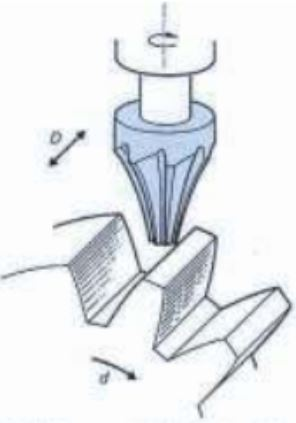
\includegraphics[width=0.5\linewidth]{Images/C1.JPG}
\end{minipage}
\begin{minipage}[t]{.44\linewidth}
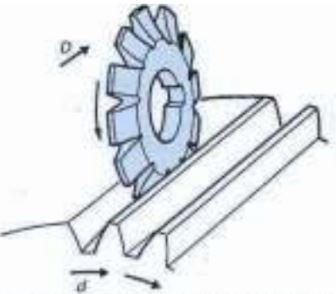
\includegraphics[width=0.7\linewidth]{Images/C2.JPG}
\end{minipage}

%%%%%%%%%%%%%%%%%%%%%%%%%%%%%%%%%%%%%%%%%%%%%%%%%%%%%%%%%%%%%%%%%%
%%%%%%%%%%%%%%%%%%%%%%%%%%%%%%%%%%%%%%%%%%%%%%%%%%%%%%%%%%%%%%%%%%%

\begin{center}



\tikzset{every picture/.style={line width=0.75pt}} %set default line width to 0.75pt        

\begin{tikzpicture}[x=0.75pt,y=0.75pt,yscale=-1,xscale=1]
%uncomment if require: \path (0,300); %set diagram left start at 0, and has height of 300

%Shape: Cube [id:dp3106942406783879] 
\draw   (163,100) -- (183,80) -- (244.55,80) -- (244.55,138) -- (224.55,158) -- (163,158) -- cycle ; \draw   (244.55,80) -- (224.55,100) -- (163,100) ; \draw   (224.55,100) -- (224.55,158) ;
%Shape: Cube [id:dp28620513900019806] 
\draw   (167,190) -- (175,182) -- (236,182) -- (236,240) -- (228,248) -- (167,248) -- cycle ; \draw   (236,182) -- (228,190) -- (167,190) ; \draw   (228,190) -- (228,248) ;
%Shape: Donut [id:dp532385415757469] 
\draw   (186,218) .. controls (186.71,211.92) and (192.22,207) .. (198.29,207) .. controls (204.37,207) and (208.71,211.92) .. (208,218) .. controls (207.29,224.08) and (201.78,229) .. (195.71,229) .. controls (189.63,229) and (185.29,224.08) .. (186,218)(180,218) .. controls (181.1,208.61) and (189.61,201) .. (199,201) .. controls (208.39,201) and (215.1,208.61) .. (214,218) .. controls (212.9,227.39) and (204.39,235) .. (195,235) .. controls (185.61,235) and (178.9,227.39) .. (180,218) ;

%Straight Lines [id:da30920672663549875] 
\draw    (506,50) .. controls (506.5,52.31) and (505.6,53.71) .. (503.29,54.2) .. controls (500.98,54.69) and (500.08,56.09) .. (500.57,58.4) .. controls (501.07,60.71) and (500.17,62.11) .. (497.86,62.6) .. controls (495.55,63.09) and (494.65,64.49) .. (495.15,66.8) .. controls (495.64,69.11) and (494.74,70.51) .. (492.43,71) .. controls (490.12,71.49) and (489.22,72.89) .. (489.72,75.2) .. controls (490.21,77.51) and (489.31,78.91) .. (487,79.4) .. controls (484.69,79.89) and (483.79,81.29) .. (484.29,83.6) .. controls (484.79,85.91) and (483.89,87.31) .. (481.58,87.8) .. controls (479.27,88.29) and (478.37,89.69) .. (478.86,92) .. controls (479.36,94.31) and (478.46,95.71) .. (476.15,96.2) .. controls (473.84,96.69) and (472.94,98.09) .. (473.44,100.4) .. controls (473.93,102.71) and (473.03,104.1) .. (470.72,104.59) -- (469.97,105.76) -- (465.63,112.48) ;
\draw [shift={(464,115)}, rotate = 302.87] [fill={rgb, 255:red, 0; green, 0; blue, 0 }  ][line width=0.08]  [draw opacity=0] (8.93,-4.29) -- (0,0) -- (8.93,4.29) -- cycle    ;
%Straight Lines [id:da36333605403726166] 
\draw    (506,50) .. controls (508.34,49.7) and (509.66,50.72) .. (509.95,53.06) .. controls (510.25,55.4) and (511.57,56.42) .. (513.91,56.12) .. controls (516.25,55.82) and (517.57,56.84) .. (517.86,59.18) .. controls (518.15,61.52) and (519.47,62.54) .. (521.81,62.24) .. controls (524.15,61.94) and (525.47,62.96) .. (525.77,65.3) .. controls (526.06,67.64) and (527.38,68.66) .. (529.72,68.37) .. controls (532.06,68.07) and (533.38,69.09) .. (533.68,71.43) .. controls (533.97,73.77) and (535.29,74.79) .. (537.63,74.49) .. controls (539.97,74.19) and (541.29,75.21) .. (541.58,77.55) .. controls (541.88,79.89) and (543.2,80.91) .. (545.54,80.61) .. controls (547.88,80.31) and (549.2,81.33) .. (549.49,83.67) .. controls (549.78,86.01) and (551.1,87.03) .. (553.44,86.73) .. controls (555.78,86.43) and (557.1,87.45) .. (557.4,89.79) .. controls (557.69,92.13) and (559.01,93.15) .. (561.35,92.85) .. controls (563.69,92.55) and (565.01,93.57) .. (565.3,95.91) .. controls (565.6,98.25) and (566.92,99.27) .. (569.26,98.97) .. controls (571.6,98.67) and (572.92,99.69) .. (573.21,102.03) -- (574.8,103.27) -- (581.13,108.16) ;
\draw [shift={(583.5,110)}, rotate = 217.75] [fill={rgb, 255:red, 0; green, 0; blue, 0 }  ][line width=0.08]  [draw opacity=0] (8.93,-4.29) -- (0,0) -- (8.93,4.29) -- cycle    ;
%Curve Lines [id:da7549614981673118] 
\draw    (282,115) .. controls (284.23,113.65) and (285.92,114.04) .. (287.09,116.19) .. controls (287.72,118.4) and (289.11,119.24) .. (291.26,118.71) .. controls (293.63,118.58) and (294.82,119.72) .. (294.82,122.15) .. controls (294.57,124.52) and (295.57,125.87) .. (297.81,126.2) .. controls (300.1,126.81) and (300.91,128.27) .. (300.24,130.58) .. controls (299.43,132.83) and (300.08,134.33) .. (302.17,135.08) .. controls (304.37,136.31) and (304.91,137.94) .. (303.79,139.97) .. controls (302.59,141.93) and (302.99,143.51) .. (304.98,144.72) .. controls (306.94,146.07) and (307.23,147.73) .. (305.86,149.7) .. controls (304.42,151.6) and (304.61,153.33) .. (306.43,154.89) .. controls (308.18,156.22) and (308.26,157.82) .. (306.66,159.69) .. controls (304.99,161.48) and (304.97,163.11) .. (306.6,164.59) .. controls (308.15,166.55) and (308.03,168.2) .. (306.24,169.55) .. controls (304.37,171.18) and (304.14,172.84) .. (305.57,174.55) .. controls (306.86,176.74) and (306.52,178.4) .. (304.57,179.55) .. controls (302.5,180.96) and (302.05,182.61) .. (303.23,184.52) .. controls (304.34,186.52) and (303.77,188.16) .. (301.53,189.43) -- (301.32,189.97) -- (298.16,196.88) ;
\draw [shift={(297,199)}, rotate = 299.74] [fill={rgb, 255:red, 0; green, 0; blue, 0 }  ][line width=0.08]  [draw opacity=0] (8.93,-4.29) -- (0,0) -- (8.93,4.29) -- cycle    ;
%Curve Lines [id:da4175170921395901] 
\draw    (70,137) .. controls (68.17,135.17) and (68.06,133.38) .. (69.66,131.61) .. controls (71.32,129.96) and (71.34,128.42) .. (69.73,126.99) .. controls (68.2,125.14) and (68.36,123.46) .. (70.22,121.93) .. controls (72.13,120.54) and (72.43,118.85) .. (71.14,116.87) .. controls (69.95,114.75) and (70.36,113.21) .. (72.38,112.24) .. controls (74.51,111.14) and (75.11,109.48) .. (74.18,107.25) .. controls (73.25,105.18) and (73.94,103.68) .. (76.25,102.74) .. controls (78.43,102.2) and (79.26,100.72) .. (78.75,98.31) .. controls (78.22,96.06) and (79.1,94.75) .. (81.39,94.38) .. controls (83.68,94.12) and (84.68,92.84) .. (84.41,90.54) .. controls (84.28,88.17) and (85.41,86.94) .. (87.8,86.83) .. controls (90.17,86.84) and (91.43,85.64) .. (91.58,83.25) .. controls (91.88,80.8) and (93.13,79.77) .. (95.32,80.15) .. controls (97.78,80.4) and (99.14,79.41) .. (99.4,77.19) .. controls (100.11,74.72) and (101.57,73.78) .. (103.8,74.37) .. controls (106,75.02) and (107.4,74.22) .. (108.01,71.99) .. controls (108.74,69.74) and (110.23,68.99) .. (112.5,69.74) .. controls (114.73,70.55) and (116.32,69.85) .. (117.26,67.63) -- (120.39,66.39) -- (127.66,63.86) ;
\draw [shift={(130.5,63)}, rotate = 163.74] [fill={rgb, 255:red, 0; green, 0; blue, 0 }  ][line width=0.08]  [draw opacity=0] (8.93,-4.29) -- (0,0) -- (8.93,4.29) -- cycle    ;
%Shape: Cube [id:dp5589972086691033] 
\draw   (382,118.01) -- (389.97,110.04) -- (414.5,110.04) -- (414.5,133.16) -- (406.53,141.13) -- (382,141.13) -- cycle ; \draw   (414.5,110.04) -- (406.53,118.01) -- (382,118.01) ; \draw   (406.53,118.01) -- (406.53,141.13) ;
%Straight Lines [id:da6766074698451421] 
\draw    (461,141) .. controls (462.78,142.55) and (462.9,144.21) .. (461.35,145.99) .. controls (459.8,147.77) and (459.92,149.43) .. (461.7,150.98) .. controls (463.48,152.52) and (463.6,154.18) .. (462.05,155.96) .. controls (460.5,157.74) and (460.62,159.4) .. (462.4,160.95) .. controls (464.18,162.5) and (464.3,164.16) .. (462.75,165.94) .. controls (461.2,167.72) and (461.32,169.38) .. (463.1,170.93) .. controls (464.88,172.47) and (465,174.13) .. (463.45,175.91) .. controls (461.91,177.69) and (462.03,179.35) .. (463.81,180.9) .. controls (465.59,182.45) and (465.71,184.11) .. (464.16,185.89) .. controls (462.61,187.67) and (462.73,189.33) .. (464.51,190.88) -- (464.73,194.03) -- (465.29,202.01) ;
\draw [shift={(465.5,205)}, rotate = 265.98] [fill={rgb, 255:red, 0; green, 0; blue, 0 }  ][line width=0.08]  [draw opacity=0] (8.93,-4.29) -- (0,0) -- (8.93,4.29) -- cycle    ;
%Shape: Cube [id:dp9274267266045786] 
\draw   (373,207.38) -- (377.64,202.74) -- (413,202.74) -- (413,236.36) -- (408.36,241) -- (373,241) -- cycle ; \draw   (413,202.74) -- (408.36,207.38) -- (373,207.38) ; \draw   (408.36,207.38) -- (408.36,241) ;
%Shape: Donut [id:dp7250755657980528] 
\draw   (384.01,223.61) .. controls (384.43,220.09) and (387.62,217.23) .. (391.14,217.23) .. controls (394.66,217.23) and (397.18,220.09) .. (396.77,223.61) .. controls (396.35,227.13) and (393.16,229.99) .. (389.64,229.99) .. controls (386.12,229.99) and (383.6,227.13) .. (384.01,223.61)(380.54,223.61) .. controls (381.18,218.17) and (386.11,213.75) .. (391.55,213.75) .. controls (396.99,213.75) and (400.89,218.17) .. (400.25,223.61) .. controls (399.61,229.05) and (394.67,233.46) .. (389.23,233.46) .. controls (383.79,233.46) and (379.9,229.05) .. (380.54,223.61) ;

%Curve Lines [id:da07916793730107075] 
\draw    (599,132) .. controls (600.9,133.55) and (601.1,135.27) .. (599.6,137.15) .. controls (598.01,138.82) and (598.08,140.47) .. (599.79,142.1) .. controls (601.46,143.89) and (601.46,145.59) .. (599.77,147.2) .. controls (598.07,148.84) and (598.03,150.55) .. (599.65,152.33) .. controls (601.26,153.92) and (601.21,155.47) .. (599.49,156.98) .. controls (597.76,158.79) and (597.69,160.55) .. (599.3,162.26) .. controls (600.91,163.99) and (600.86,165.68) .. (599.14,167.33) .. controls (597.44,168.73) and (597.41,170.33) .. (599.04,172.12) .. controls (600.69,173.91) and (600.67,175.55) .. (599,177.04) .. controls (597.34,178.87) and (597.36,180.55) .. (599.05,182.06) .. controls (600.76,183.86) and (600.81,185.57) .. (599.2,187.18) .. controls (597.61,188.83) and (597.71,190.56) .. (599.49,192.36) .. controls (601.27,193.81) and (601.4,195.4) .. (599.89,197.13) .. controls (598.4,198.92) and (598.58,200.52) .. (600.43,201.93) -- (600.98,205.79) -- (602.43,213.52) ;
\draw [shift={(603,216)}, rotate = 256.37] [fill={rgb, 255:red, 0; green, 0; blue, 0 }  ][line width=0.08]  [draw opacity=0] (8.93,-4.29) -- (0,0) -- (8.93,4.29) -- cycle    ;
%Curve Lines [id:da3369110243924378] 
\draw  [dash pattern={on 4.5pt off 4.5pt}]  (606,243) .. controls (608.88,259.32) and (604.85,271.95) .. (599.21,285.32) ;
\draw [shift={(598.5,287)}, rotate = 293.2] [color={rgb, 255:red, 0; green, 0; blue, 0 }  ][line width=0.75]    (10.93,-3.29) .. controls (6.95,-1.4) and (3.31,-0.3) .. (0,0) .. controls (3.31,0.3) and (6.95,1.4) .. (10.93,3.29)   ;

% Text Node
\draw  [fill={rgb, 255:red, 155; green, 155; blue, 155 }  ,fill opacity=0.39 ]  (11,145) -- (124,145) -- (124,183) -- (11,183) -- cycle  ;
\draw (14,149) node [anchor=north west][inner sep=0.75pt]  [font=\footnotesize] [align=left] {On a analyser notre\\dessin de définition};
% Text Node
\draw  [fill={rgb, 255:red, 155; green, 155; blue, 155 }  ,fill opacity=0.35 ]  (135,38) -- (270,38) -- (270,76) -- (135,76) -- cycle  ;
\draw (138,42) node [anchor=north west][inner sep=0.75pt]  [font=\footnotesize] [align=left] {\begin{minipage}[lt]{89.36pt}\setlength\topsep{0pt}
On sait quelles sont les surfaces à usiner\end{minipage}};
% Text Node
\draw (252,107) node [anchor=north west][inner sep=0.75pt]  [font=\footnotesize] [align=left] {Brut};
% Text Node
\draw (243,211) node [anchor=north west][inner sep=0.75pt]  [font=\footnotesize] [align=left] {Pièce voulue};
% Text Node
\draw  [fill={rgb, 255:red, 155; green, 155; blue, 155 }  ,fill opacity=0.4 ]  (412.32,10) -- (606.32,10) -- (606.32,48) -- (412.32,48) -- cycle  ;
\draw (509.32,29) node  [font=\footnotesize] [align=left] {\begin{minipage}[lt]{129.29pt}\setlength\topsep{0pt}
En fonction des surfaces à générer sur la pièce voulue\end{minipage}};
% Text Node
\draw    (598.5, 120) circle [x radius= 19.09, y radius= 12.02]   ;
\draw (586,113.5) node [anchor=north west][inner sep=0.75pt]  [font=\footnotesize] [align=left] {Tour};
% Text Node
\draw    (464.5, 127) circle [x radius= 40.31, y radius= 12.02]   ;
\draw (437,120.5) node [anchor=north west][inner sep=0.75pt]  [font=\footnotesize] [align=left] {Fraiseuse};
% Text Node
\draw    (605.5, 229) circle [x radius= 40.31, y radius= 12.02]   ;
\draw (578,222.5) node [anchor=north west][inner sep=0.75pt]  [font=\footnotesize] [align=left] {Fraiseuse};
% Text Node
\draw  [fill={rgb, 255:red, 155; green, 155; blue, 155 }  ,fill opacity=0.4 ]  (624.82,144.5) -- (683.82,144.5) -- (683.82,165.5) -- (624.82,165.5) -- cycle  ;
\draw (654.32,155) node  [font=\footnotesize] [align=left] {Phase 10};
% Text Node
\draw  [fill={rgb, 255:red, 155; green, 155; blue, 155 }  ,fill opacity=0.4 ]  (623.82,107.5) -- (684.82,107.5) -- (684.82,128.5) -- (623.82,128.5) -- cycle  ;
\draw (654.32,118) node  [font=\footnotesize] [align=left] {Exemple :};
% Text Node
\draw  [fill={rgb, 255:red, 155; green, 155; blue, 155 }  ,fill opacity=0.4 ]  (624.82,249.5) -- (683.82,249.5) -- (683.82,270.5) -- (624.82,270.5) -- cycle  ;
\draw (654.32,260) node  [font=\footnotesize] [align=left] {Phase 40};
% Text Node
\draw  [fill={rgb, 255:red, 155; green, 155; blue, 155 }  ,fill opacity=0.4 ]  (624.82,168.5) -- (683.82,168.5) -- (683.82,189.5) -- (624.82,189.5) -- cycle  ;
\draw (654.32,179) node  [font=\footnotesize] [align=left] {Phase 20};
% Text Node
\draw  [fill={rgb, 255:red, 155; green, 155; blue, 155 }  ,fill opacity=0.4 ]  (624.82,194.5) -- (683.82,194.5) -- (683.82,215.5) -- (624.82,215.5) -- cycle  ;
\draw (654.32,205) node  [font=\footnotesize] [align=left] {Phase 30};
% Text Node
\draw  [fill={rgb, 255:red, 155; green, 155; blue, 155 }  ,fill opacity=0.44 ]  (367.82,156.5) -- (426.82,156.5) -- (426.82,177.5) -- (367.82,177.5) -- cycle  ;
\draw (397.32,167) node  [font=\footnotesize] [align=left] {Phase 10};
% Text Node
\draw    (468.5, 220) circle [x radius= 51.62, y radius= 12.02]   ;
\draw (433,213.5) node [anchor=north west][inner sep=0.75pt]  [font=\footnotesize] [align=left] {Pièce voulue};


\end{tikzpicture}
\end{center}

%%%%%%%%%%%%%%%%%%%%%%%%%%%%%%%%%%%%%%%%%%%%%%%%%%%%%%%%%%%%%%%%%%%%
%%%%%%%%%%%%%%%%%%%%%%%%%%%%%%%%%%%%%%%%%%%%%%%%%%%%%%%%%%%%%%%%%%



\section{Désignation des outils}
\subsection{Les outils en tournage}
\subsection{Les outils en fraisage}


\begin{exo}\label{exo1} En vous aidant de la Figurindiquez d'où viennent les ordres de déplacement des machines outils.\end{exo}

%%%%%%%%%%%%%%%%%%%%%%%%%%%%%%%%%%%%%%%%%%%%%%%%%%%%%%%%%%%%%%%%%%%%%%%%%%%%%%%%%%%%%%
%%%%%%%%%%%%%%%%%%%%%%%%%%%%%%%%%%%%%%%%%%%%%%%%%%%%%%%%%%%%%%%%%%%%%%%%%%%%%%%%%%%%%%
%%%%%%%%%%%%%%%%%%%%%%%%%%%%%%%%%%%%%%%%%%%%%%%%%%%%%%%%%%%%%%%%%%%%%%%%%%%%%%%%%%%%%%

\begin{tcolorbox}[colback=blue!5!white,colframe=red!75!black]
  \bcinfo szldkjfvhspdjfnmzekjfnmlsqdkjfnmlskdjfnlksmqdjf
\end{tcolorbox}


\section{ANNEXE}
\begin{tcolorbox}[colback=blue!5!white,colframe=orange!75!black]
\begin{center}
    \textbf{Glossaire :}
\end{center}
\begin{itemize}
    \item CNC : Computer Numerical Control (Commande numérique par calculateur);
    \item MOCN : Machine Outil à commande numérique, elle est programmable et équipée d'une "commande numérique par calculateur" (CNC). Elle est en général dédiée à des fabrication variées de pièces différentes, lancées en petits lots répétitifs.
    \item CU : Centre d'usinage : En fait, c'est une MOCN qui est complétée d'autres équipement périphériques qui assurent notamment : \begin{itemize}
        \item le changement automatique d'outils stockés dans des magasins d'outils;
        \item le changement automatique de pièce (palettisation)
        \item éventuellement le convoyage des copeaux (convoyeur)
    \end{itemize}
    Il est dédié à des fabrications variées de pièces différentes.
    \item CAO : Conception Assistée par Ordinateur;
    \item FAO : Fabrication Assistée par Ordinateur.
\end{itemize}
\end{tcolorbox}


\begin{figure}
\centering
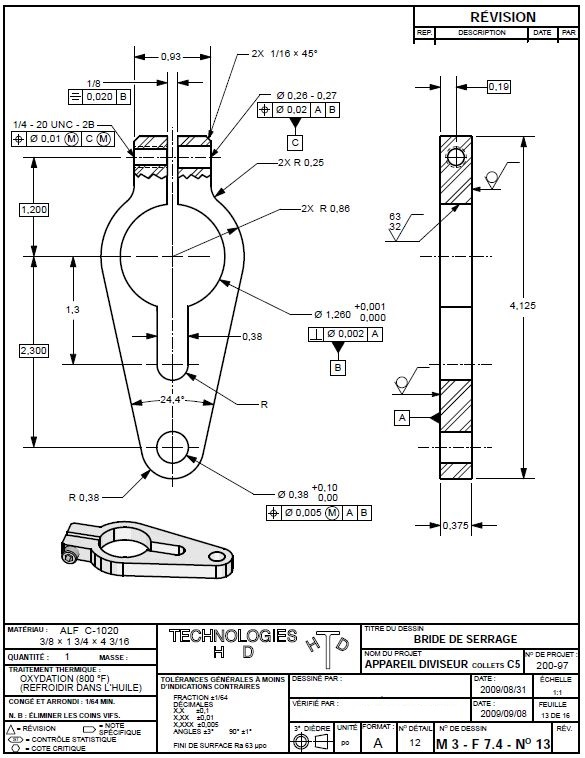
\includegraphics[width=0.9\linewidth]{Images/dessin1.JPG}
\caption{Dessin de définition d'une bride de serrage}
\label{bride}
\end{figure}




\begin{figure}
\centering
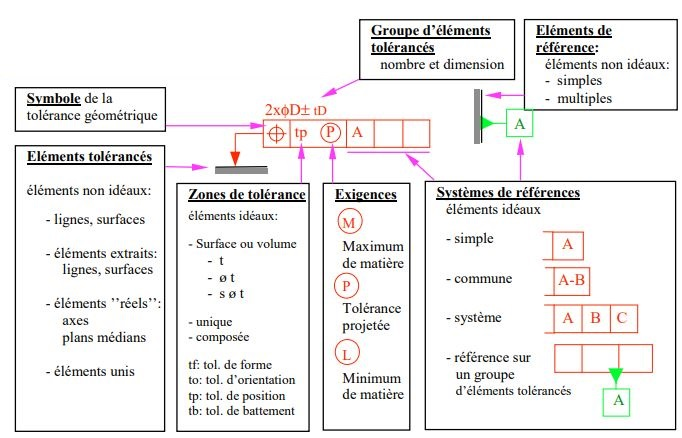
\includegraphics[width=0.9\linewidth]{Images/gps.JPG}
\caption{Aide mémoire pour spécification géométrique}
\label{gps}
\end{figure}




\end{document}

